\documentclass[12pt, a4paper]{ctexart}

\usepackage{booktabs}
\usepackage{graphicx}
\usepackage{amsmath}
\usepackage{mathcomp}
\usepackage{mathabx}
\usepackage{enumitem}
\usepackage[colorlinks,linkcolor=red,urlcolor = blue]{hyperref}
\usepackage{fancyhdr}
\fancypagestyle{plain}{
\fancyhead{}
\renewcommand{\headrulewidth}{1pt}
\fancyfoot{}
\fancyhead[L]{\thepage}
\fancyhead[R]{\leftmark}
}
\usepackage[top=1.5in,bottom=1.5in, left=1in, right=1in]{geometry}

\makeatletter
\newcommand{\rmnum}[1]{\romannumeral #1}
\newcommand{\Rmnum}[1]{\expandafter\@slowromancap\romannumeral #1@}
\makeatother

\ctexset{
    % 修改 section
    section={   
        name={,},
        number={\chinese{section}},
        format=\heiti\raggedright
    },
    % 修改 subsection
    subsection={   
        name={(,)},
        number={\chinese{subsection}},
        format=\heiti
    }
}

\begin{document}
\title{测量金属的杨氏模量}
\author{唐晨宇 \quad 2300934207}
\date{2024年3月22日}

\maketitle

\begin{abstract}
	利用梁的弯曲测量金属梁的杨氏模量,并进行数据处理,分析主要误差来源并说明实验中部分系统误差来源,并作较深入的讨论。
\end{abstract}
	
\tableofcontents

\clearpage

\pagestyle{headings}

\section{实验原理}
核心公式:
\[
	\lambda = \frac{mgl^3}{4Eah^3}
\]

参考吕斯骅《新编基础物理实验》基础实验\Rmnum{1}\quad 实验八

\section{仪器用具}
\begin{description}
	\item[钢尺] 用于测量金属梁有效长度,最小分度0.1cm
	\item[游标卡尺] 用于测量金属梁宽度,最小分度0.05mm
	\item[千分尺] 用于测量金属梁厚度,最小分度0.01mm
	\item[读数显微镜] 用于测量挠度,最小分度0.1cm
	\item[电子天平] 用于测量砝码质量,允差0.06g
\end{description}

\section{原始数据}
\begin{itemize}
	\item 金属梁有效长度$l = 27.85cm$(单次测量)\quad $\sigma_l = \frac e{\sqrt3} = 0.06cm $

	\begin{table}[htbp]
    \centering
    \caption{金属梁宽度$a$ \quad 测量数据记录表}
    \begin{tabular}{cccccccc}
	\toprule
    $i$     & 1     & 2     & 3     & 4     & 5     & 平均值$\bar{a}$   & 不确定度$\sigma_{aA}$  \\
    \midrule
    $a/mm$  & 14.90 & 14.90 & 14.95 & 14.93 & 14.90 & 14.92 & 0.01 \\
	\bottomrule
    \end{tabular}%
    \label{tab:t1}%
    \end{table}%

	\item 金属梁宽度$\bar{a} \pm \sigma_{\bar{a}} = (14.92 \pm 0.03)mm$ \\
    其中$\displaystyle{\sigma_{\bar{a}} = \sqrt{\sigma_{aA}^2 + (\frac{e_{aB}}{\sqrt{3}})^2 } = 0.05mm}$
	\footnote{所有B类不确定度均取仪器最小分度。}
	\footnote{不妨假设误差均匀分布,故计算时应除以$\sqrt3$。} \\

    \begin{table}[htbp]
    \centering
    \begin{tabular}{cccccccc}
    \toprule
    $i$     & 1      & 2     & 3     & 4     & 5     & 平均值$\bar{h}$ & 不确定度$\sigma_{hA}$ \\
    \midrule
    $h/mm$  & 1.530  & 1.523 & 1.531 & 1.514 & 1.532 & 1.526 & 0.0034 \\
    \bottomrule
    \end{tabular}%
	\caption{金属梁厚度$h$ \quad 测量数据记录表}
    \label{tab:t2}%
    \end{table}%

    \item 金属梁厚度$(\bar{h} - h_0) \pm \sigma_{\bar{h}} = (1.528 \pm 0.007)mm $ \\
    其中$\displaystyle{\sigma_{bar{h}} = \sqrt{\sigma_{hA}^2 + (\frac{e_{aB}}{\sqrt{3}})^2 } = 0.007mm}$ \\
	$h_0 = -0.002mm$为千分尺零位读数

    \begin{table}[htbp]
    \centering
    \caption{金属梁挠度$\lambda$-负载质量$m$测量数据记录表}
    \begin{tabular}{ccccccc}
    \toprule
    $i$   & $\Delta m_i/g $ &$m_i/g $    & $x_i/mm$ & $x'_i/mm$ & $\lambda/mm$ & $\lambda'/mm$ \\
    \midrule
    0     & ——     & 0.00    & 45.5  & 45.4  & 0.0  & 0.0 \\
    1     & 200.39 & 200.39  & 44.6  & 44.5  & 0.9  & 0.9 \\
    2     & 199.56 & 399.95  & 43.7  & 43.6  & 1.8  & 1.8 \\
    3     & 200.94 & 600.89  & 42.8  & 42.7  & 2.7  & 2.7 \\
    4     & 200.66 & 801.55  & 41.9  & 41.8  & 3.6  & 3.6 \\
    5     & 200.08 & 1001.63 & 41.0  & 40.9  & 4.5  & 4.5 \\
    6     & 200.13 & 1201.76 & 40.1  & 40.0  & 5.5  & 5.4 \\
    \bottomrule
    \end{tabular}%
    \label{tab:t3}%
    \end{table}%

	\item 挠度$\lambda$与金属梁负载质量$m_i$之间关系
	
\end{itemize}

\section{数据处理}
\subsection{最小二乘法计算结果}

\[
	\lambda = \frac{gl^3}{4Eah^3}m_i = km_i \quad \Rightarrow \quad E = \frac{gl^3}{4kah^3}
\]

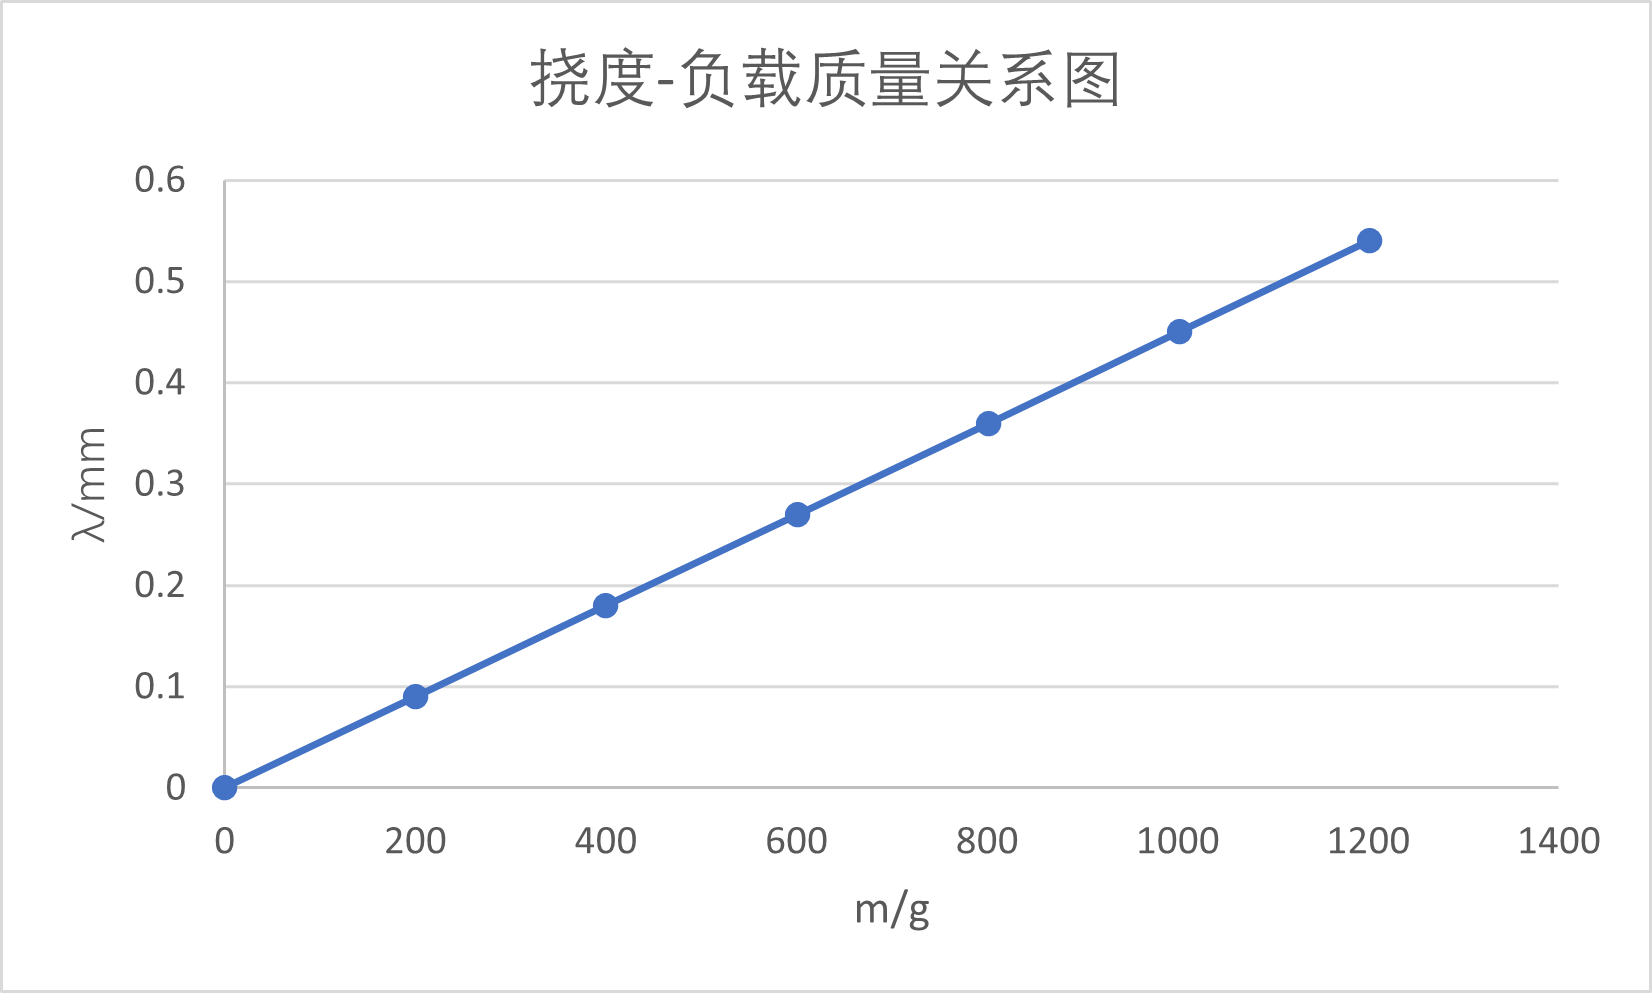
\includegraphics[]{挠度-负载质量线性关系.png}

通过最小二乘法线性拟合,得到二者关系:\\
\[
    k = 4.4925\times 10^{-3}m/kg \qquad r = 0.99999976
\]
\[
    \sigma_k = k \sqrt{\frac{\frac1{r^2}-1}{n-2}} = 0.0014\times 10^{-3}m/kg
\]
最终计算可得$\overline{E} = 2.213 \times 10^{11} Pa $\\
由于$\lambda$与$\lambda'$几乎没有区别,故仅计算一组数据,不再重复计算。


\subsection{最小二乘法误差分析}
由不确定度叠加法则:
\[
    \frac{\sigma_{\overline{E}}}{\overline{E}} = \sqrt{(3\frac{\sigma_l}l)^2 + (\frac{\sigma_{k}}{k})^2 + (\frac{\sigma_{\bar{a}}}{\bar{a}})^2 + (3\frac{\sigma_{\bar{h}}}{\bar{h}})^2}
    = 0.016
\]
\[
    \Rightarrow \quad \sigma_{\overline{E}} = 0.035 \times 10^{11}Pa
\]

最终结果为$(\overline{E} \pm \sigma_E) = (2.213 \pm 0.035)\times 10^{11}Pa$

\subsection{逐差法计算结果}
由于$\lambda$过于均匀,我们可以直接得到$\delta \lambda = 0.9mm $

由表\ref{tab:t3}可知$\displaystyle{\overline{\Delta m} = 200.29g \quad \sigma_{\overline{\Delta m}} = \sqrt{\sigma_{A}^2 + (\frac{e_{B}}{\sqrt{3}})^2 } = 0.20g} $
\[
    \overline{E} = \frac{\Delta mgl^3}{4\delta \lambda ah^3} = 2.2129\times 10^{11}Pa
\]

\subsection{逐差法误差分析}
将间接计算得到的斜率不确定度$\sigma_{k}$转化为直接得出的$\sigma_{\overline{\Delta m}}$和$\sigma_{\delta \lambda}\equiv 0$
\[
    \frac{\sigma_{\overline{E}}}{\overline{E}} = \sqrt{(3\frac{\sigma_l}l)^2 + (\frac{\sigma_{\overline{\Delta m}}}{\overline{\Delta m}})^2 + (\frac{\sigma_{\bar{a}}}{\bar{a}})^2 + (3\frac{\sigma_{\bar{h}}}{\bar{h}})^2}
    = 0.016
\]
\[
    \Rightarrow \quad \sigma_{\overline{E}} = 0.035 \times 10^{11}Pa
\]

最终结果仍为$(\overline{E} \pm \sigma_E) = (2.213 \pm 0.035)\times 10^{11}Pa$

\section{结论分析}
\subsection{方案对比}
从最终结果中我们可以看出两种数据处理方法在该实验条件下得出的结论几乎完全相同。
分析各项数据可以得出,其主要原因是由于梁的弯曲程度较小,在读数显微镜精度有限的条件下,相应的挠度不易精确测量,导致挠度变化无法反映出砝码质量的微小误差
(大约$1g/200g = 0.5\% $的误差)。
在当前实验条件下,作为因变量的挠度变化的精度仅有一位有效数字,无法匹配自变量$m_i$五位有效数字的变化。

相应的,$m_i$的误差在3\textpertenthousand 量级,而$\Delta m$的误差在1 \textperthousand 量级。
二者的差距由于挠度$\lambda$接近1/10的巨大误差而无法在结论中体现,故两种方法得出了几乎完全相同的结论。

\subsection{误差主要来源}
虽然挠度的测量存在较大误差,但显然在当前实验条件下斜率拟合引起的误差并非误差的主要来源——相对误差仅为$\frac{\sigma_k}k = $3\textpertenthousand 且在结果中以-1次出现。
与此同时,宽度$a$和有效长度$l$的相对误差均在3\textperthousand 量级,厚度$h$的相对误差在5\textperthousand 量级,总体相差不多,
但由于$l$和$h$在结果计算公式中以3次方的形式出现,通过误差传递被放大了接近一个数量级,因此二者成为了主要的误差来源。

\subsection{系统误差}
由于实验系统引起的误差是多方面的,其中最主要、值得探讨的有以下三个方面:
\begin{enumerate}
    \item[一] 由于金属梁两端刀片的不平行和用于悬挂砝码的金属框上的刀片磨损导致的挠度读数不准以及金属梁受力不均。
    
    两端刀片不平行对有效长度$l$的测量误差有非常大的影响,而由于三次方的存在对最终实验的结果也会有较大的影响。
    若二者之间存在$3^{\circ}$的夹角,刀片长度为2cm,则$l$就会产生一个0.1cm量级的变化,相应产生的相对误差在3\textperthousand 量级,即相对误差增加了近一倍!
    挠度读数误差的影响在当前条件下由于仪器精确度较低而被减弱了,但在更加精确的测量中这将成为一个不可忽视的因素。
    刀片不平行、金属框未放置在金属梁中央、装置整体倾斜\footnote{参见\ref{appendix:附录B}} 和刀片磨损均会使金属梁受力不均,不同情况对实验结果的影响不同,但均会导致数据偏离线性。
    这里需要较为深入的理论推导计算,在本实验精度下也没有明显的体现(通过钢尺对齐可以尽量减小不平行程度),因此不予细究。
    \item[二] 由于金属梁的生锈、老化而导致的数据偏离线性。
    \item[三] 由于金属框质量的作用。
    
    悬挂砝码的金属框本身具有一定质量,但本实验中数据是线性的,因此理论上这一因素并不会对数据产生影响,反而在加上砝码之前对金属梁做了一个预拉伸的工作,对实验后续工作有一定帮助。
    但结合上面两点,由于存在装置和梁在各方向的倾斜以及其悬挂位置相对中心位置的偏离,金属框的质量会产生更大的摩擦,从而助长了梁的非线性弯曲。
\end{enumerate}

从以上几点可以看出,较低的精度限制了这一实验的操作和数据处理方式,但当精度提高时也会随之产生多种非线性效应,从而导致更大的误差。
可见在进行物理量的测量时要选择合适精度的量具,在有限条件内采用最合适、最精确的数据处理方式,才能得出较为合理且精确的实验结果。

\appendix
\section{原始实验记录}
详见\href{https://github.com/oFtangcY/experiment-I/blob/main/1.8%E6%9D%A8%E6%B0%8F%E6%A8%A1%E9%87%8F/origin%20data.pdf}{实验记录}

若打不开Github页面,当前文件后附原始实验记录。

包含CCD及弯曲梁两种测量方法实验结果。

\section{金属梁整体倾斜引发的测量误差分析}
\label{appendix:附录B}
画示意图太费时间了,暂时先不画,之后有机会再说。

总之如果两侧刀片高度不同导致的横向倾斜,会使测量的挠度偏小(斜边与直角边的关系)。
由于推导过程中忽略金属梁本身的重力(即忽略金属梁内部应力),故暂且不考虑倾斜产生摩擦力引起的应力变化。
因此仅考虑挠度偏小,最终结果是会偏大的。举例来说,若倾斜角度为$5^\circ$,挠度测量会产生4\textperthousand 的误差(在当前实验条件下显然是体现不出来的)。
\end{document}
